%!TEX program=xelatex

\documentclass[11pt]{ctexart}  
\usepackage[top=2cm, bottom=2cm, left=2cm, right=2cm]{geometry}  
\usepackage{algorithm}  
\usepackage{algorithmicx}  
\usepackage{algpseudocode}  
\usepackage{amsmath}  
\usepackage{graphicx}
\usepackage{amsmath}
\usepackage{amssymb}
\usepackage{enumerate}
\usepackage{booktabs}

\floatname{algorithm}{算法}
\renewcommand{\algorithmicrequire}{\textbf{输入:}}  
\renewcommand{\algorithmicensure}{\textbf{输出:}} 

\title{密码学实验报告8}
\author{张天辰 17377321}

\makeatletter
\newenvironment{breakablealgorithm}
  {% \begin{breakablealgorithm}
   \begin{center}
     \refstepcounter{algorithm}% New algorithm
     \hrule height.8pt depth0pt \kern2pt% \@fs@pre for \@fs@ruled
     \renewcommand{\caption}[2][\relax]{% Make a new \caption
       {\raggedright\textbf{\ALG@name~\thealgorithm} ##2\par}%
       \ifx\relax##1\relax % #1 is \relax
         \addcontentsline{loa}{algorithm}{\protect\numberline{\thealgorithm}##2}%
       \else % #1 is not \relax
         \addcontentsline{loa}{algorithm}{\protect\numberline{\thealgorithm}##1}%
       \fi
       \kern2pt\hrule\kern2pt
     }
  }{% \end{breakablealgorithm}
     \kern2pt\hrule\relax% \@fs@post for \@fs@ruled
   \end{center}
  }
\makeatother

\begin{document}
\maketitle{}



\section{ECC实现Diffie-Hellman密钥交换}
\subsection{ECC上相关计算及其实现} % (fold)
完成所有ECC上密码算法的前提是实现ECC上的基本运算,包括点的加减法以及点与数的数乘运算。

椭圆曲线$E(F_q)$上点的加法有如下规则:
\begin{enumerate}[1]
    \item $P + O = P$。这条基本不会用到。
    \item $P + -P = O$,其中若$P = (x, y)$,则$-P = (x, -y)$。这条规则使得$P - Q = P + (-Q)$,因此可以通过加法直接实现减法。
    \item 一般地,设$P + Q = R$,则
    $$R_x = \lambda^2 - P_x - Q_x \mod q$$
    $$R_y = \lambda(P_x - R_x) - P_y \mod q$$
    其中
    $$
    \lambda = \left\{
    \begin{aligned}
    & \frac{3P_x^2 + a}{2P_y} \mod q \\
    & \frac{Q_y - P_y}{Q_x - P_x} \mod q 
    \end{aligned}
    \right.
    $$
\end{enumerate}

在Python语言中,这一步操作可以重载运算符。算法实现如下:
\begin{breakablealgorithm} 
    \caption{ECC加减法}
    \begin{algorithmic}[1] %每行显示行号  
        \Function{add}{$P, Q$}
            \If {$P == Q$}
                \State $\lambda \gets ((3 * P_x^2 + a) *$\Call{reverse}{$2 * P_y$}$) \% q$
            \Else
                \State $\lambda \gets ((Q_y - P_y) *$\Call{reverse}{$Q_x - P_x$}$) \% q$
            \EndIf
            \State $x = (\lambda * \lambda - P_x - Q_x) \% q$
            \State $y = (\lambda * (P_x - x) - P_y) \% q$
            \State \Return $(x, y)$
        \EndFunction
        \Function{sub}{$P, Q$}
            \State \Return \Call{add}{$P, (Q_x, -Q_y)$}
        \EndFunction
    \end{algorithmic}
    \end{breakablealgorithm}

而在椭圆曲线上的数乘运算$Q = nP$实际上就是$n$个$P$相加,但是如果单纯地用循环的方法相加,显然效率太低。从上述的$P, Q$中恢复$n$的问题称为椭圆曲线上的“离散对数问题”,这不由得让人想到有一些“幂”运算的特征。事实上,这里的算法确实可以采用类似快速幂算法的方式,即将$n$写成二进制形式,然后根据其每一位为1或0进行操作。如果是1就将当前结果数乘2(自己加自己),然后再和$P$相加;如果是0就仅仅数乘2。这样就大量简化了运算。

算法实现如下:
\begin{breakablealgorithm} 
    \caption{ECC数乘}
    \begin{algorithmic}[1] %每行显示行号  
        \Function{multi}{$P, n$}
            \State $b \gets n$转化为二进制后从第二位开始的比特串
            \State $result \gets P$
            \For {each $i \in b$}
                \If {$i == 1$}
                    \State $result = result + result$
                    \State $result = result + P$
                \Else
                    \State $result = result + result$
                \EndIf
            \EndFor
            \State \Return $result$
        \EndFunction
    \end{algorithmic}
    \end{breakablealgorithm}
% subsection ecc上相关计算及其实现 (end)
\subsection{ECCDH密钥交换协议及其实现} % (fold)
ECCDH交换协议流程如下:A和B共享一条椭圆曲线及其生成元$G$以及$G$的阶$n$。A和B各自从$[1, n - 1]$中选取随机数$n_A, n_B$作为私钥,然后A发送给B$P_A = n_A \times G$,B发送给A$P_B = n_B \times G$。基于等式$n_A \times P_B = n_B \times P_A = K$,双方可以共享密钥$K$。想破解这个协议就要解决椭圆曲线上的离散对数问题,这被认为是困难的。

算法实现如下:
\begin{breakablealgorithm} 
    \caption{ECCDH}
    \label{alg_dh}
    \begin{algorithmic}[1] %每行显示行号  
        \Function{generateKey}{}
            \State $private \gets rand(1, n - 1)$
            \State $public \gets $\Call{multi}{$G, private$}
        \EndFunction
        \Function{calcKey}{$P_B$}
            \State $sharedKey \gets $\Call{multi}{$P_B, private$}
        \EndFunction
    \end{algorithmic}
    \end{breakablealgorithm}
% subsection 密钥交换协议的实现 (end)
\section{ECC实现ElGamal密码体制} % (fold)
\subsection{算法原理} % (fold)
变量名延续上节的定义。用户私钥$n_A$为$[1, n-1]$中的一个数,公钥$P_A$为$n_A \times G$。设需要加密的信息可以写为椭圆曲线上的点$P$,则加密时首先生成随机数$k \in [1, n-1]$,然后令$C_1 = k \times G$,$C_2 = P + k \times P_A$。$C_1, C_2$为密文。其原理就是先利用$k$和$P_A$掩盖$M$,再利用$C_1$掩盖$k$。想要去除掩盖,除非拥有私钥,否则必须解椭圆曲线上离散对数问题。解密时,根据等式$k \times P_A = n_A \times C_1$,就可以利用$P = C_2 - n_A \times C_1$得到明文。
% subsection 算法原理 (end)
\subsection{算法实现} % (fold)
\begin{enumerate}
    \item 密钥生成
    参考DH协议里的密钥生成方法,即算法\ref{alg_dh}中的函数\Call{generateKey}{}。

    \item ElGamal加解密
    \begin{breakablealgorithm} 
    \caption{ElGamal}
    \begin{algorithmic}[1] %每行显示行号  
        \Function{encrypt}{$P$}
            \State $k \gets rand(1, n - 1)$
            \State \Return (\Call{multi}{$G, k$}, $P + $\Call{multi}{$P_A, k$})
        \EndFunction
        \Function{decrypt}{$C_1, C_2$}
            \State \Return $C_2 - $\Call{multi}{$C_1, n_A$}
        \EndFunction
    \end{algorithmic}
    \end{breakablealgorithm}
\end{enumerate}
% subsection 算法实现 (end)
\subsection{算法测试} % (fold)
\begin{figure}[htbp]
\centering
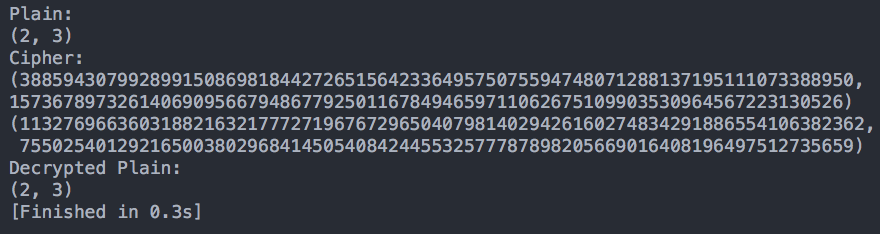
\includegraphics[width=13.20cm, height=3.51cm]{elgamal.png}
\caption{ElGamal测试}
\label{img_elgamal}
\end{figure}
% subsection 算法结果 (end)
% section ElGamal加解密 (end)
\section{国密SM2算法} % (fold)
\subsection{SM2算法原理} % (fold)
SM2是对简单椭圆曲线密码体制的改进。其密钥生成和前述的ElGamal体制相同,但加解密过程就相对复杂一些。\textbf{尽管算法标准中将很多操作规定为在比特串上进行,但是考虑到计算机读写文件都以字节为单位,而且使用字节串并不影响其本身的逻辑,还更加节省空间。因此这里都采用字节串进行实现。比特串的应用场景应该是硬件实现,而不是软件。}

沿用之前的符号定义,如果要加密字节串$M$,长度为$klen$,则要先生成随机数$k \in [1, n - 1]$,并且令$C_1 = k \times G$转换为字节串后的结果。此后令$(x2, y2) = k \times P_A$,并将$x2, y2$转化为字节串后拼接在一起为$x2||y2$。令$T = KDF(x2||y2, 8 * klen)$,其中KDF为密钥派生函数,会在稍后介绍。如果$T$全为0,就重新选$k$。此后令$C_2 = M \oplus T$。再令$C_3 = Hash(x2 || M || y2)$,这里的Hash函数论理应当是SM3等国密算法,但这里用sha-256代替。

解密时,根据等式$k \times P_A = n_A \times C_1$,就可以利用私钥恢复$(x2, y2)$,从而恢复$T$,则有$M = T \oplus C_2$。$C_3$的Hash函数值用于验证完整性。

接下来介绍KDF函数,其输入本为一个整数,但在函数里也要转成比特串,于是本方案考虑直接输入字节串,减少无谓的类型转换。此外还要输入一个预定的输出位数。其函数逻辑为,定义一个32位计数器$ct$,每次将其拼接在输入字节串$Z$的后面,然后送入Hash函数,并拼接在以前的输出之后,此后$ct$自增1。这样的操作持续到位数足够,并截断最后的位数以凑整输入的比特长度。
% subsection sm2算法原理 (end)
\subsection{SM2算法实现} % (fold)
密钥生成参考DH协议里的密钥生成方法,即算法\ref{alg_dh}中的函数\Call{generateKey}{}。
\begin{breakablealgorithm} 
\caption{SM2}
\begin{algorithmic}[1] %每行显示行号
    \Function{KDF}{$Z, klen$}
        \State 因为采用sha-256,因此$v \gets 256$
        \State $ct \gets 1$
        \For {each $i \in [1, klen/v]$}
            \State $hashList \gets hashList || Hash(Z || ct)$
            \State $ct \gets ct + 1$
        \EndFor
        \State 从右边截断$hashList$若干位,直到它长度为$klen$位。
        \State \Return $hashList$
    \EndFunction
    \Function{encrypt}{$plainList$}
        \State $klen \gets $\Call{len}{$plainList$}
        \State $k \gets $\Call{randint}{$[1, n - 1]$}
        \State $c1 \gets $\Call{multi}{$G, k$}
        \State $(x2, y2) \gets $\Call{multi}{$public, k$}
        \State $t \gets $\Call{KDF}{$x2 || y2, 8 * klen$}
        \State 如果$t == 0$,则返回12
        \State $c2 \gets plainList \oplus t$
        \State $c3 \gets $\Call{Hash}{$x2 || plainLlist || y2$}
        \State \Return $c1 || c3 || c2$
    \EndFunction
    \Function{decrypt}{$cipherList$}
        \State $cipherList$前65字节为$c1$,中间32字节为$c3$,其余为$c2$
        \State $klen \gets $\Call{len}{$c2$}
        \State $(x2, y2) \gets$\Call{multi}{$private, c1$}
        \State $t \gets $\Call{KDF}{$x2 || y2, 8 * klen$}
        \State $m \gets c2 \oplus t$
        \State $u \gets $\Call{Hash}{$x2 || m || y2$}
        \If {$u \neq c3$}
            \State 报错
        \EndIf
        \State \Return $m$
    \EndFunction
\end{algorithmic}
\end{breakablealgorithm}
% subsection sm2算法实现 (end)
\subsection{算法测试} % (fold)
算法明文文件默认为主程序同一文件夹下的Plain.txt,密文文件默认为同一文件夹下的Cipher.txt。在程序开始时会询问是否生成密钥,如果是则生成一对公私钥,否则沿用已有的(如果有)。如图\ref{img_sm2},尽管我们无法从程序输出看到具体运行信息,但我们还是可以看到,至少解密得到的文件通过了Hash检验。
\begin{figure}[htbp]
\centering
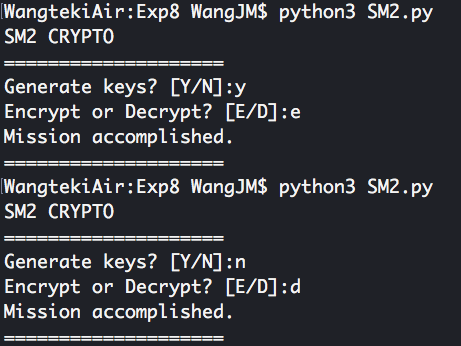
\includegraphics[width=9.22cm, height=6.92cm]{sm2.png}
\caption{SM2程序运行图}
\label{img_sm2}
\end{figure}[htbp]

然后我们再更改Plain.txt的后缀为.jpg,可以看到这实际上是一张图片,解密成功。
\begin{figure}
\centering

\includegraphics[width=9.8cm, height=10.5cm]{plain.png}
\caption{解密后明文}
\label{img_plain}
\end{figure}
% subsection 算法测试 (end)
% section 国密sm2算法 (end)
\section{感想} % (fold)
本次实验我对椭圆曲线上的加解密算法进行了实现。实际上,非对称加密可能比起对称算法要好实现一些,毕竟加解密方式都比较干脆,不像对称密码那样操作很多。在实现SM2的过程中我也尝试进行了一些优化,比如通过更改数据类型提高速度、更换更快的函数等等。

在实现了SM3后,我会将这里的Hash函数换成SM3,实现技术独立(笑)。
% section 感想 (end)
\end{document}